\section{3G modul}

Enhedstest af 3G modulet foregår ved test af PUT og GET request, som er de metoder der er implementeret på dronen.

For udelukkende at have fokus på 3G modulet under enhedstesten, testes der ikke op imod den server som ellers anvendes til projektet. I stedet benyttes hjemmesiden requestb.in[X], en hjemmeside der der tillader test af HTTP kommunikation. Ved at tilgå Requestb.in og starte en session tildeles en URL der kan bruges til test. Requestbin indsamler information om alle HTTP request lavet til den tildelte URL. 

På figur \ref{fig:get_req} vises et GET request der sendes fra 3G modulet til en requestb.in server. Den første linje efter \textit{data:} fortæller om requestet er gennemført succesfuldt eller ej. Svaret \textit{200 ok} betyder at GET requestet er gået igennem og det ønskede data på korrekt vis er hentet. 

\vspace{0.3cm}

\begin{figure}[H]
\centering
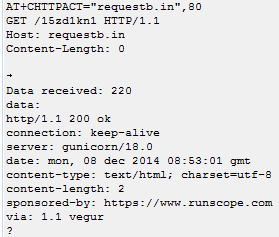
\includegraphics[width=0.5\textwidth]{Billeder/Test/get_requestbin.png}
\caption{GET Request}
\label{fig:get_req}
\end{figure}

\newpage

PUT request bruges til at sende data til eller opdatere information på server. 
På figur \ref{fig:putrequest_module} vises et PUT der sendes fra 3G modulet til requestb.in. De føreste seks linjer på figur \ref{fig:putrequest_module} viser requestet header med linje syv er requestet body. 

\begin{figure}[H]
\centering
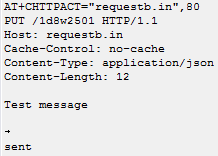
\includegraphics[width=0.5\textwidth]{Billeder/Test/putrequest_module.png}
\caption{PUT metode}
\label{fig:putrequest_module}
\end{figure}

\vspace{1cm}

På figur \ref{fig:put_req} vises det information der tilgængelig på server efter PUT requestet er fuldført. \textit{RAW BODY} viser det data der er modtaget og HEADERS indeholder parametrene for HTTP protokollen.

\begin{figure}[H]
\centering
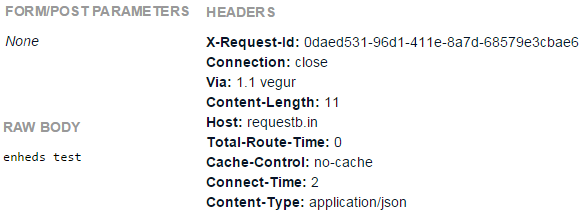
\includegraphics[width=0.8\textwidth]{Billeder/Test/put_request.png}
\caption{Information på server}
\label{fig:put_req}
\end{figure}
